%!TEX TS-program = xelatex
%!TEX encoding = UTF-8 Unicode

\documentclass[tikz]{standalone}
\usetikzlibrary{positioning}

\begin{document}
  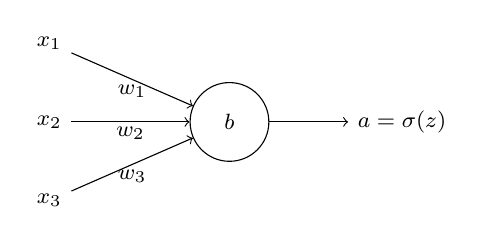
\begin{tikzpicture}[
    neuron/.style={circle,draw,inner sep=0pt,minimum size=10mm},
    font=\footnotesize
    ]

    \node (neuron) [neuron] {$b$};
    \node (x2) [left=1.5 of neuron] {$x_2$};
    \node (x1) [left=1.5 of neuron,yshift=1cm] {$x_1$};
    \node (x3) [left=1.5 of neuron,yshift=-1cm] {$x_3$};
    \node (output) [right=of neuron] {$a = \sigma(z)$};

    \draw[->] (x1) to node [above,yshift=-3.5mm] {$w_1$} (neuron);
    \draw[->] (x2) to node [above,yshift=-3.5mm] {$w_2$} (neuron);
    \draw[->] (x3) to node [above,yshift=-3.5mm] {$w_3$} (neuron);
    \draw[->] (neuron) to (output);

  \end{tikzpicture}
\end{document}
